\documentclass[12pt]{article}
\usepackage[margin=1in]{geometry}
\usepackage{amsmath, amssymb, amsthm}
\usepackage{tcolorbox}
\usepackage{lastpage}
\usepackage{fancyhdr, accents}
\usepackage{natbib}
\usepackage{graphicx}
\usepackage{hyperref}

\pagestyle{fancy}
\setlength{\headheight}{40pt}

\newcommand{\ubar}[1]{\underaccent{\bar}{#1}}

\newcommand\tab[1][1cm]{\hspace*{#1}}

\title{CSC110Y1-F Fall 2020 - Fundamentals of Computer Science 1 \\ Course Project Proposal}
\author{
  Ching Chang\\
  \and
  Letian Cheng\\
  \and
  Arkaprava Choudhury\\
  \and
  Hanrui Fan
}
\date{\today}

\begin{document}

\maketitle

\newpage

\lhead{Ching Chang, Letian Cheng \\ Arkaprava Choudhury, Hanrui Fan}
\rhead{CSC110Y1-F Fall 2020 \\ Fundamentals of Computer Science 1 \\ Course Project Proposal}
\cfoot{\thepage\ of \pageref{LastPage}}

\begin{enumerate}
\item \section*{Part 1}
\textbf{An interactive report of the effect of Amazon rainforest's area on the local annual precipitation and $CO_2$ emission (with python prime shipping).}

Ching Chang, Letian Cheng, Arkaprava Choudhury, Hanrui Fan

\newpage

\item \section*{Part 2}

\begin{text}
Research Question: \textbf{To what extent do the changes in the Amazon rainforest’s area affect the local annual precipitation and $CO_2$ emission?}

During our initial research on topics related to climate change, we found that the South American rainforest contributes 20\% \citep{Tho20} of the oxygen produced by photosynthesis on land,
while the Amazon rainforest is responsible for 10\% of the current greenhouse gas emissions \citep{Mel93}.
This information was surprising to us since 20\% of photosynthesis implies a lot of conversion from carbon dioxide,
which is a greenhouse gas, to oxygen, whereas the 10\% contribution to greenhouse gas seems to contradict that information.
Due to this contradiction, we were curious about whether tree populations actually help control the climate.
After some research, we learned that the effect of trees on climate change is more complex than we originally thought.
There are many factors to consider, such as the carbon dioxide to oxygen conversion, the tendency to trap heat due to their dark color,
reaction to form methane and ozone, and political movements revolving around tree plantations \citep{Mar20}.
This led us into choosing an empirical approach —we wanted to directly observe the relationship between the change of tree population and climate change.
We chose to focus our data on the Amazon rainforest not only because it is the largest rainforest on Earth \citep{WWF13},
but also because there have been several pieces of evidence that show that the Amazon rainforest has been suffering from deforestation recently. Although there might be other underlying factors causing the changes in precipitation and $CO_2$ emission, it is still worth considering that over $700,000 km^2$ ($270,000 mi^2$) of Amazon rainforest had been lost since 1970, reducing its size to 80.7\% of its original size, in 2018 \citep{But20};
There have been more than 40,000 fires in the rainforest in 2019 \citep{Gov20}; and that forest exploitation in Amazon has risen for 14 consecutive months in June 2020 \citep{Reu20}.
With these major pieces of evidence of deforestation correlating to the change in global and local climate, we believe that it is a relevant topic to contemporary society that should not be ignored.
\end{text}

\newpage

\item \section*{Part 3}

\begin{itemize}
    \item \textbf{TRMM (TMPA/3B43) Rainfall Estimate L3 1 month 0.25 degree x 0.25 degree V7 (TRMM\_3B43)}

    This is a rainfall estimate dataset made by NASA.\newline
    we have download the data for reviewers:

    https://sudo.fit/3B43\_rainfall.zip

    If you want to download by yourself, the link is here:\newline
    https://disc.gsfc.nasa.gov/datasets/TRMM\_3B43\_7/summary

    \item \textbf{annual CO2 emissions by region}

    This is a CO2 emissions data provided by ``our world in data".\newline
    The link is here:\newline
    https://ourworldindata.org/grapher/annual-co-emissions-by-region

    \item \textbf{Deforestation Figures for the Amazon}

    This is a deforestation data provided by ``mongabay".\newline
    The link is here\newline
    https://rainforests.mongabay.com/amazon/deforestation\_calculations.html
\end{itemize}
\newpage

\item \section*{Part 4}

\begin{text}

PROCESSING INPUT DATA

In the input part, we first start the deserialization by creating a class called \texttt{Climate} with public attribute \texttt{name}, \texttt{year} and \texttt{value} to maintain the entire input data section can be saved in the same format for later analysing with data from different types (e.g. HDF and CSV).

In our own method \texttt{precipitation\_read\_hdf}, we first processed the input selected latitude and longitude of the top left endpoint and bottom right endpoint of the rectangular region in the global map. Since the NASA data is stored as longitude and latitude every 0.25 degrees. The longitude is recorded as 1440 points, while the latitude NASA only stores from 50 degrees north to 50 degrees south i.e. 400 points\citep{N3B43}. We used the knowledge of linear algebra to change the basis and represent the input endpoint latitudes and longitudes with the new basis.
Then we import \texttt{os} library to visit all the HDF file in the folder path by method \texttt{os.listdir} to get a list of all HDF file name\citep{PytOS}. To read HDF file, we import a new library called \texttt{pyhdf}. This library helps to get access to the precipitation dataset from NASA since NASA use HDF to save all the satellite data. We mainly use \texttt{SD} and \texttt{SDC} class in \texttt{pyhdf.SD} module since \texttt{SD} helps to open a HDF file and return SD Instance and \texttt{SDC} is used to call \texttt{SDC.READ} method to use \textbf{read only mode} with HDF file\citep{Pyhdf}. We also use \texttt{numpy} library to deal with array transpose with imported dataset \citep{Pynpy}.

In our own function \texttt{precipitation\_read\_csv} and \texttt{deforestation\_read\_csv}, we only import \texttt{csv}, we use \texttt{DictReader} to get the header of the CSV file\citep{Pycsv}. Then the corresponding value in the CSV will be read through \texttt{for loop} and in each loop iteration create a \texttt{Climate} instance and stored in a list.

We include a function \texttt{get\_data()} to give the example location of the file saved and the endpoints we select. This function also returns a list containing all three types of data(Co2emission/Precipitation/Deforestation).

Function \texttt{save\_data\_as\_csv} is a serialization process. We transform \texttt{Climate} class into a CSV file that is being merged and updated. And then in the analysis process, the merged data can be simply used by function \texttt{read\_data\_from\_csv} which is also a deserialization process.


ANALYSIS DESCRIPTION.

For this project, we use smooth polynomial fitting to relate two of the variables in our \texttt{nested list}. Now, although there exist readily available functions that would do the same in the module \texttt{numpy} \citep{Sci20}, we try implementing our own functions for the same, to test our learning from the course.

We split the mathematical algorithm for this problem using top-down design. The most important part of the data analysis section is the PolynomialRegression custom class that we have defined, which, when initializing a variable of this class, takes in a dictionary with the name of the independent variable as the key, and its corresponding value in the dictionary as the list of all its values, and also, a corresponding dictionary for the dependent variable, and also a specified degree for the polynomial, and the level of precision expected.

Now, earlier, we were initially experiencing errors in the final result, as the values were quite large and the functions used some approximations which were resulted in non-negligible errors. So, we switched to using the `relative polynomial regression model', i.e., the values relative to the maximum of the values, and effectively, `scale' the range and domain of the polynomial to simply $[0, 1]$, which has the outcome of a better approximation of a trend but a more indirect polynomial equation relating the two variables. As such, we had to include some more calculations in our class methods. For example, to evaluate the predicted value at a certain point, if $x_{max}, y_{max}$ were the maximum $x,y$ values, then we had to convert from the absolute $x$-value to the relative $x$-value (by dividing by $x_{max}$), then determine the relative $y$-value, and convert it to the absolute $y$-value (by multiplying by $y_{max}$). Another good example is the \texttt{get\_instantaneous\_slopes()} method, where we had to translate the chain rule of derivatives into code. To explain, let $Y$ be the relative $y$-model, and let $X$ be the relative $x$-model. Then, by the chain rule, we have,
\begin{align*}
    \frac{dy}{dx} &= \frac{y_{max}}{x_{max}} \cdot \frac{dY}{dX}
\end{align*}

The initializer then calls upon a function that we designed using the ordinary least squares method to create a list of coefficients for the polynomial function that has the least variance with respect to the input data. Note that this list is implemented in terms of ascending order of power, to favour the implementation of the other methods in this class that analyze how well this polynomial represents the data (i.e., a measure of the accuracy of this polynomial). We defined the method \texttt{\_\_call\_\_} to allow the polynomial to defined as a callable, i.e., if \texttt{poly} is a variable of type PolynomialRegression, we we can simply evaluate \texttt{poly} at a value \texttt{x} by calling \texttt{poly(x)}.

We first have the method \texttt{r\_squared} to calculate the coefficient of determination for this polynomial. We also have \texttt{extreme\_absolute\_error} to return the maximum and minimum absolute difference between the polynomial's value and a particular value in the input data. Then, we have the additional methods \texttt{covariance\_with\_polynomial} and \texttt{correlation\_of\_data} as additional measure of accuracy.

The other part in this section of the project is defining our own functions to handle the matrices involved in such a computation. We tried defining our own functions for these operations as much as possible, and while these implementations are not as efficient as possible, they serve our purposes quite well. For one, any improvement will be rather negligible as the degrees we consider are rather small, so the matrix size doesn't change rapidly; and also, optimizing the algorithm would lead to reducing the running time by only a few milliseconds, which is not our main priority in this code. However, if we wished to optimize these functions, we could either choose to use the \texttt{matmul()} function in the \texttt{numpy} module, or we could choose to implement parts of the matrix multiplication with dot products by using \texttt{numpy.dot()} function from the \texttt{numpy} module to improve the process.

We have the functions \texttt{make\_matrix} and \texttt{find\_coefficients} which are perhaps the most important functions in this part. The former initializes the matrix $X$, and the latter solves the matrix equation $\vec{y} = X\vec{\beta} + \epsilon$ for $\beta$, where $X$ represents the matrix of powers of $x$ created from the input data, $\vec{y}$ represents the values of $y$ in the input data, and $\vec{\beta}$ is the estimated coefficients vector, while $\vec{\epsilon}$ consists of the random errors at each of the points (i.e., the difference between the polynomial evaluated at the point and the actual $y$-value). Since we could not find any efficient way to create an algorithm to compute the inverses (we haven't really covered any such `efficient' algorithm in either MAT223 or MAT240), we made use of \texttt{numpy}'s built-in function called \texttt{numpy.linalg.inv()} along with a type conversion method \texttt{tolist()} that converts objects of type array (a data class in \texttt{numpy}) to a nested list format.

Finally, we added a method in the PolynomialRegression class to allow for plotting the graph of the polynomial and a scatter plot of the data, using the functions \texttt{numpy.linspace} and \texttt{matplotlib.pyplot}, and specifying our own customizations to the graph.

INTERACTIVE PART

Our program also includes an interactive text-based model because the graphing library we use does not allow us to search for specific values. We thought that a text-based output would be more appropriate if the user is looking for the coefficient of determination, or the rate of change at a specific data point, because the graphical representation of those values would not be useful to the user.

The interactive model first calls \texttt{prompt\_independent} and \texttt{prompt\_dependent} to get the desired independent and dependent variables for our calculation. Note that the possible independent variables are $CO_2$ and forest area, and the possible dependent variables are $CO_2$ and precipitation. Therefore, if $CO_2$ is chosen as the independent variable, our program would not prompt the user for the dependent variable. Our program also does not prompt the user for the degree of the polynomial regression line, because we have plotted each degree ourselves beforehand and noticed that degree 3 is the most appropriate degree for these graphs. As a result, we hard-coded the program to use degree 3 every time to reduce weights on the user-end.

After selecting the variables and finishing the calculation, the interactive model uses a while loop with a condition that is always True. This allows the user to be prompted as many times as they wish. Inside of the while loop, we prompt the user again for the values they want to look up using \texttt{prompt\_y} and \texttt{prompt\_x}, which each has a while loop inside that iterates until the user input is valid.

After obtaining the variables to look for, the program would iterate through every value in the list of values the user is searching for. For example, if the user wants to find the forest cover when the year is 2000, the program would iterate through the list of years. If any of the values \textit{is close} (using \texttt{math.isclose()}) to the expected value, in this case, 2000, we take the dependent value (forest cover) with the same index in the list of dependent values. To do so, we need a list of values for each variable, and the index of each value in the list must match the other. This is achieved using the function \texttt{get\_output\_data()}, which retrieves the required values we need from \texttt{PolynomialRegression} and \texttt{get\_data}.

\end{text}

\newpage

\item \section*{Part 5}

\begin{text}

\textbf{Special instruction for pyhdf:}
You can't install pyhdf directly using pip. Please follow the following instructions:

https://fhs.github.io/pyhdf/install.html

Make sure the HDF4 library or included files are in directories that are searched by default on your system (in the PATH). You can install pypdf using pip if the HDF4 library is already in your PATH.

If you don't want to install pyhdf, you can just read from our parsed data (dataset.csv). Use read\_data\_from\_csv in get\_data\_nohdf.py. It will return a list contains Climate classes, which we will use later in the data analysis.

\textbf{TRMM (TMPA/3B43) Rainfall Estimate L3 1 month 0.25 degree x 0.25 degree V7 (TRMM\_3B43)}

We have downloaded and uploaded on one of our members' server. It is nearly 1G. Here is the link:

http://sudo.fit/3B43\_rainfall.zip

If you decide to download by yourself, please follow the instruction provided by NASA:

https://disc.gsfc.nasa.gov/datasets/TRMM\_3B43\_7/summary

Please unzip it into a folder called 3B43\_rainfall.

\textbf{Annual total CO2 emissions, by world region}

Their website provided the option to download them as csv.

https://ourworldindata.org/grapher/annual-co-emissions-by-region

It is called ``annual-co-emissions-by-region.csv" in MarkUs.
You can manually do it, too.

\textbf{Deforestation Figures for the Amazon}

The original form is here:

https://rainforests.mongabay.com/amazon/deforestation\_calculations.html

We have changed this into csv manually. It is called ``deforestation.csv" in markus.
You can manually do it, too.

\textbf{Pre-processing of the datasets}

All the data are saved into a class called Climate. It havs 3 valuables: name, year and value.

We serialized our data. They are saved in dataset.csv. To transform the raw dataset into the serialized data, please use get\_data.py and call save\_data\_as\_csv(get\_data(), ``dataset.csv").

If you want to deserialize from the transformed dataset, use

read\_data\_from\_csv(``dataset.csv") in get\_data\_nohdf.py

\textbf{After download, please put all the data file into ./data/3B43\_rainfall. The final data folder should looks like:
}

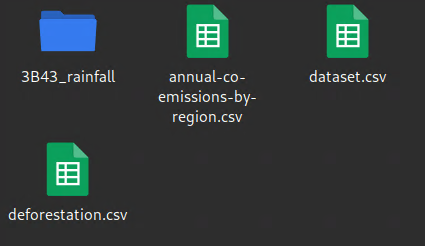
\includegraphics[scale=0.5]{./datafolder.png}

\textbf{inside ./data/3B43\_rainfall should looks like:}

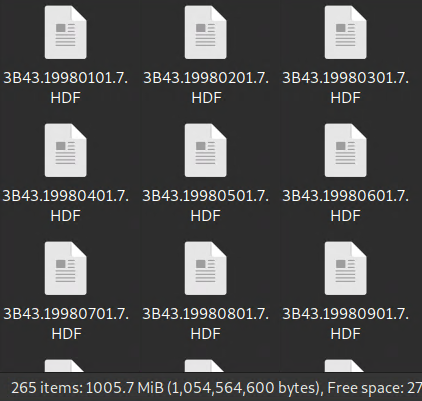
\includegraphics[scale=0.5]{./rainfallfolder.png}

\textbf{Getting output}

Run \texttt{main.py}. The console will prompt you for the independent variable to use for the calculation. You can either choose \texttt{`forest cover'} or \texttt{`CO2'}. If you choose \texttt{`CO2'}, the only dependent variable is \texttt{`precipitation'}, so the program will not prompt you for the dependent variable. However, if you choose \texttt{`forest cover'}, the program will prompt you again for the dependent variable, which could either be \texttt{`CO2'} or \texttt{`precipitation'}.

After choosing the variables, the program will start asking you for a variable you want to search for, and the value of another variable where you want it. For example, if you want to search for the value of forest cover in the year of 2000, input forest cover for the first prompt, and year=2000 for the second prompt. We've also provided an example when prompting you, so hopefully it is clear.

When you are done with the text-based report, just press ctrl + C on windows or cmd + C on mac to kill the process, and an interactive graph will appear (it might appear in the background so check other windows). You can use the magnifying glass and select a portion to zoom in on, or the 4-directional arrow symbol to move the graph. Hovering over the graph will show you the x and y coordinates below the graph.

\end{text}



\newpage

\item \section*{Part 6}

\begin{text}

In the input part, our original plan was to grab and parse the data directly from the website via a python program and store it in a file. At the time we didn't have a firm idea of the format of the storage. And we found that one of the datasets was so small that we didn't think it was necessary to write long code to grab this little bit of data. We stored the deforestation data as CSV files by manual processing. Another thing we did not expect is that the rainfall data is not divided by country, but by latitude and longitude. Also this dataset has the most special storage type. So we first need to find a python library that can open this type of file and process the corresponding data type \texttt{ndarray} that it outputs\citep{Pynpy}. Second, we needed to process the selected area. We chose to pick the top-left endpoint and the bottom-right endpoint of the rectangular region of the Amazon directly from the map. The rest of the input part procedure followed the original design in our proposal.

For the data analysis part of this project, we initially planned on using an approach that was quite similar to the calculus `way' of constructing the polynomial regression (hereby shortened to simply `polyreg') model. For instance, in the project proposal, we mentioned that we would first construct a trivial initial candidate polynomial (we were, of course, referring to the linear regression model from Assignment 1, when we said trivial, since it has the right `shape' but nor the right degree), which would then use to find the sum of the squares of the perpendicular distance from each of the points to the polynomial. We had also mentioned that we would then minimize this sum by using the simplex algorithm.

However, we later found out that coding the simplex algorithm and modifying it to fit this task was not a manageable feat, as there so many degrees of freedom for this problem that we simply could not write an efficient piece of code to work in all cases.

As such, we switched our approach to the more `linear algebra way' of solving this task, by using matrices instead. We made good use of the Gauss-Markov theorem \citep{Gmthrm11}, and applied it to the ordinary least squares method \citep{Ols} to arrive at a relatively straightforward, already well-established, and mathematically proven approach that was more guaranteed to offer a good estimate for the polynomial model.

Because of the limited data size, we've also decided that extrapolation would not be appropriate, as the given inputs are not enough to make an accurate enough prediction. As we saw with the case for some of the polynomials we encountered when testing with randomly generated data points, the behaviour of the polynomial strayed away from the general trend as we moved away from the region of the original data.

Furthermore, we decided to remove the trivia log in our interactive model after analyzing the data and finding out that there is not much trivia. However, we also added more features in the interactive model to balance this decrease in features. For example, we added the flexibility for the user to choose which independent and dependent variable they wish to use for the calculation. We also added more values for the user to look up, namely the absolute error of the regression line at each x value.

\end{text}

\newpage

\item \section*{Part 7}

\begin{text}

%Do the results of your computational exploration help answer this question?
%What limitations did you encounter, with the datasets you found, the algorithms/libraries you used, or other obstacles?
%What are some next steps for further exploration?

\emph{\textbf{Do the results of your computational exploration help answer this question?}}

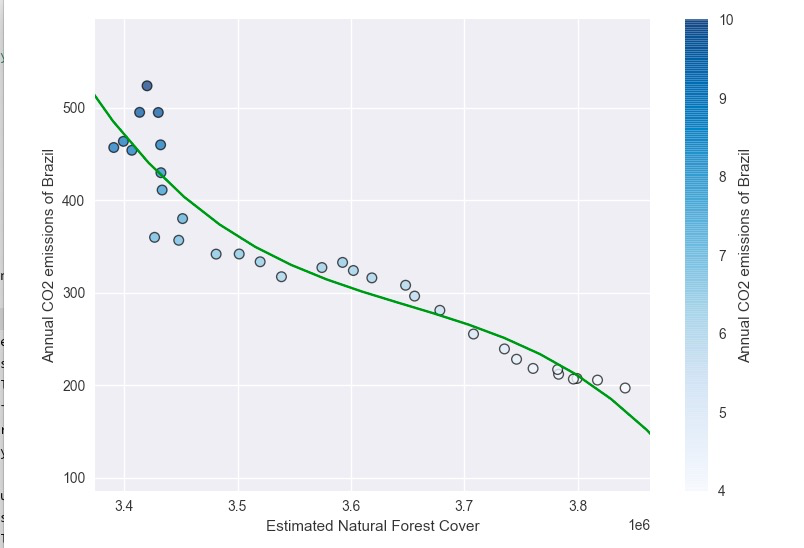
\includegraphics[scale=0.5]{./co2-vs-forest.png}

The coefficient of determinant ($r^2$) of the regression line is 0.9044761966743734, which suggests that the Estimated Natural Forest Cover has a fairly close relationship with Annual CO2 emissions of Brazil. As the forest area increases, the annual CO2 emission decreases logarithmically. This suggests that forestation does help reducing CO2 on a local level. However, this relationship could also be falsely induced by modernization in the Brazil forests. The decrease in forest cover could be caused by the use of tree-cutting machines, and could lead to more factories in the forest — both are factors that contribute to CO2 emission. Although we cannot assume that the emission of CO2 is directly affected by the forest area, our analysis helps us conclude that there exists a logarithmic relationship between the two variables. Whether this relationship is direct or indirect, manipulating the forest cover has statistically shown its effect on CO2 emission.

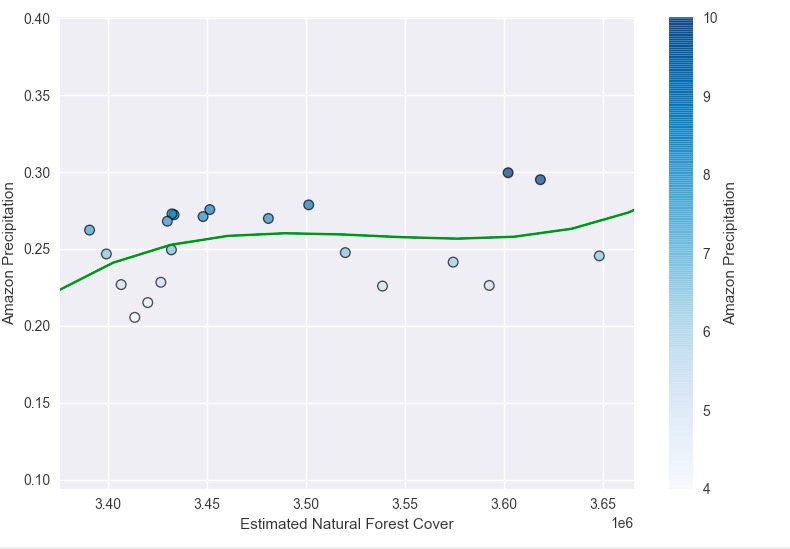
\includegraphics[scale=0.5]{./precip-vs-forest.png}

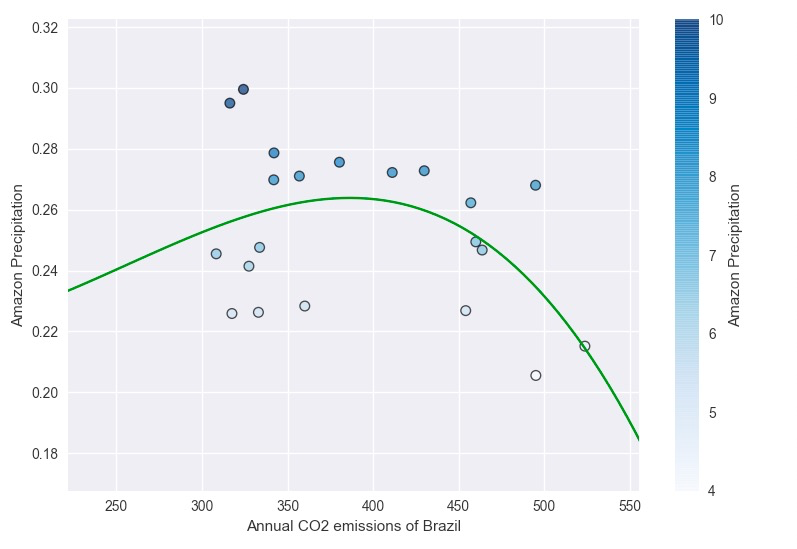
\includegraphics[scale=0.5]{./precip-vs-co2.png}

On the other hand, the Precipitation did not show a strong enough relationship with either Estimated Natural Forest Cover nor Annual CO2 emissions of Brazil, which has the r2 of 0.08946573309429795 and 0.21188218240490897 respectively. This suggests that the impact of forest cover on precipitation is negligible with the presence of other factors.

\emph{\textbf{What limitations did you encounter, with the datasets you found, the algorithms and libraries you used, or other obstacles?}}

Another significant obstacle we faced was the unity of data structure among the group. For people spending more time with calculation, the Polynomial class we created ourselves was better to work with. However, it was quite different to know what the original data structure we downloaded, and from what the data should look like at the end. We resolved this conflict by creating a public interface first, that is, Climate class. We all agreed on using this public interface, so we can easily integrate with other's code. Also, we don't need to wait until others finish before we begin our job, because we can expect the result class of our partners' code.

In terms of computation, there is an issue in the way numpy approximates the inverse of a matrix. Since computers cannot accurately handle fractions, irrationals, and polynomials, when calling the \texttt{matrix\_inverse\_numpy} function, the computer is prone to floating point error at each step in the calculation. Since the values we were dealing with differed by a large margin (for instance, forest cover was of the order of $10^6$, while precipitation was of the order of $10^{-1}$), this meant that the resulting polynomials were not as accurate as they would have been if we opted for a more manual approach of calculation, due to possible errors in the approximations used in the function \texttt{matrix\_inverse\_numpy}. To fix this, we considered the `relative polynomial regression model', i.e., the values relative to the maximum of the values, and effectively, `scale' the range and domain of the polynomial to simply $[0, 1]$, which has the outcome of a better approximation of a trend but a more indirect polynomial equation relating the two variables.

\emph{\textbf{What are some next steps for further exploration?}}

After learning that forest cover is logarithmically related to CO2 emission on a local level, we are curious about the reason. Although it makes sense that CO2 emission decreases as forest cover increases due to photosynthesis, the logarithmacity is not explained. We want to look further into this by investigating forests of different sizes and examining the change in CO2 emission as a correlated effect of the change of forest size. Moreover, we are interested in applying this knowledge in our society. For example, knowing that the emission of CO2 decreases logarithmically, should we encourage urban tree plantation as opposed to forestation, since increasing the forest size of the smaller forests yields a greater rate of change? Or maybe it is only logarithmic within the data we analyzed, and it shows a different trend on smaller forests so forestation is still more effective than urban tree plantation in terms of decreasing CO2.

Nevertheless, our current findings suggests that we can at least focus on going in the direction of encouraging tree plantation and preventing deforestation, before investigating which is more efficient for the climate in our future exploration.

\end{text}


\maketitle

\newpage

\bibliography{references}
\bibliographystyle{apalike}

\end{enumerate}

\end{document}
